\chapter{Uživatelské rozhraní}
\label{chap:ui}

Uživatelské rozhraní (anglicky \textit{User Interface}, zkráceně UI) je vrstva systému, která zajišťuje komunikaci mezi uživatelem a aplikací nebo zařízením \cite{smashing-ui}. Cílem každého uživatelského rozhraní je prezentace informací a poskytnutí nástrojů pro manipulaci se systémem. Tyto systémy jsou mnohdy zaměřeny na skupiny lidí různých národností a různých zaměření, jejichž cílem je rychlá, efektivní a intuitivní práce. Úkolem kvalitního uživatelského rozhraní je cílové skupině lidí tyto vlastnosti poskytovat.

Návrh uživatelského rozhraní však nezahrnuje pouze rozložení jednotlivých prvků a vizuální stránku systému. Důležitým prvkem je také zvolení správných prvků a nástrojů se kterými uživatelé manipulují. I v případě, že uživatel pracuje se systémem poprvé musí určité elementy působit povědomě.

\section{Grafické uživatelské rozhraní}
\label{sec:gui}

Grafické uživatelské rozhraní (anglicky \textit{Graphical User Interface}, zkráceně GUI) je typ uživatelského rozhraní, které umožňuje jednoduchou práci s elektronickým zařízením nebo aplikací. Tato vlastnost je zajištěna použitím vhodných prvků, které napomáhají lidem v orientaci a poskytují intuitivní nástroje (např. použití vhodných ikonek, tlačítek, oken atd.).

\begin{figure}[htbp]
    \centering
    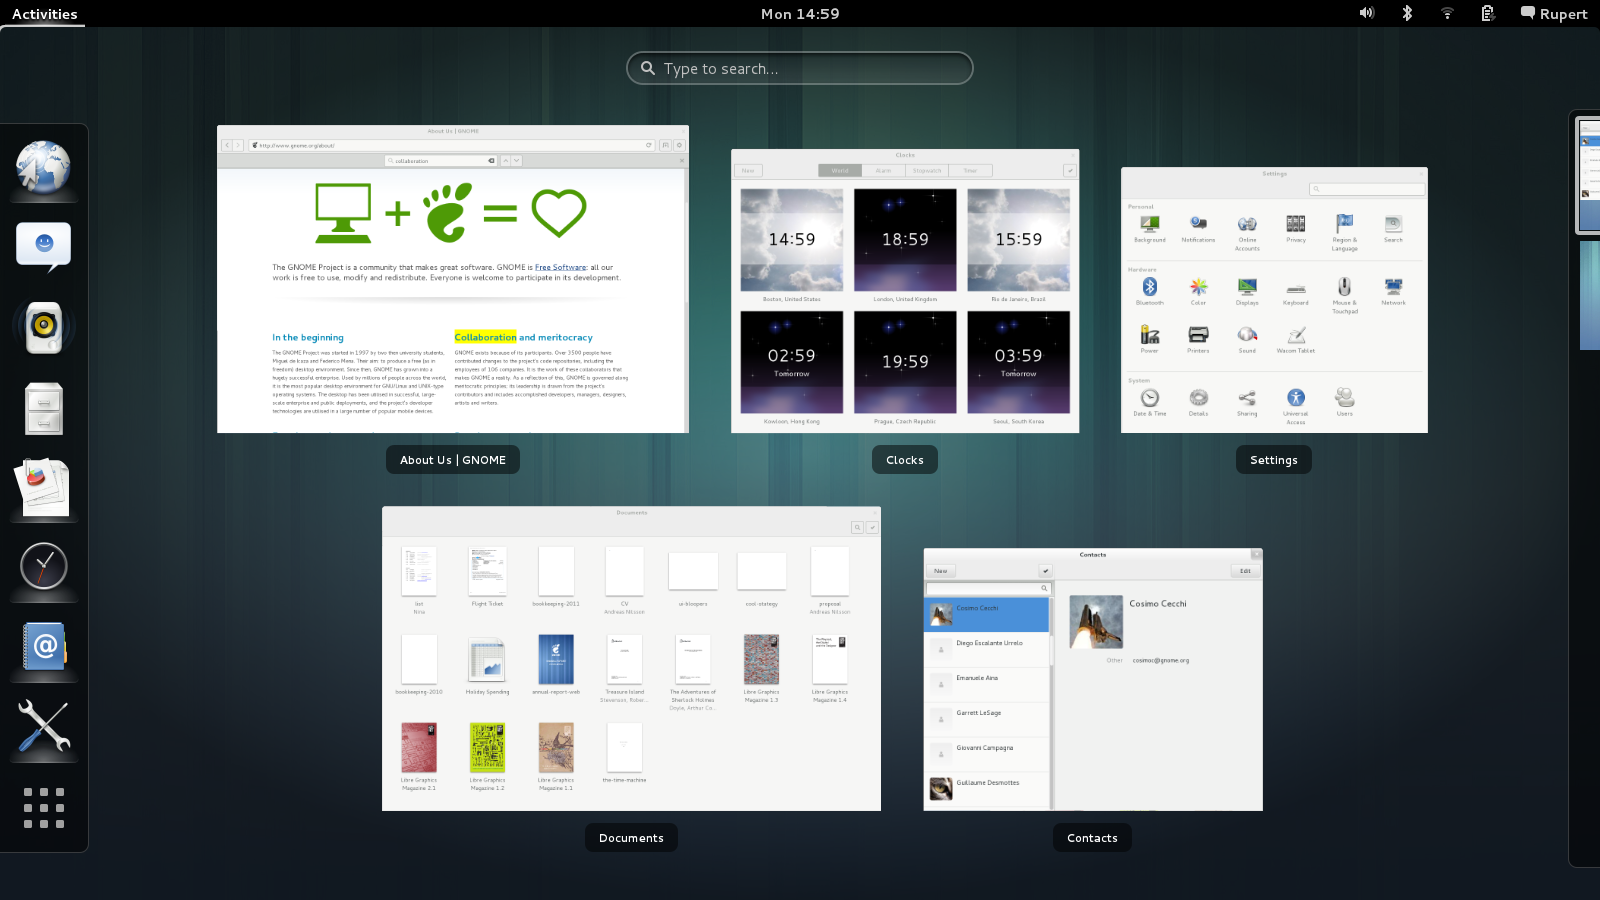
\includegraphics[width=11cm]{images/gui-example.png}
    \caption{Příklad grafického uživatelského rozhraní (TODO: zdroj -- gnome-shell).}
\end{figure}

Na vývoj grafických uživatelských rozhraní má vliv mnoho aspektů mezi něž patří mimo jiné i způsob interakce člověka s počítačem. Už na začátku osmdesátých let se začali objevovat první polohovací zařízení, díky kterým se postupně eliminovaly nedostatky textových rozhraní---především jejich nemožná integrovatelnost mezi běžné uživatele. Tím vznikla základní podoba WIMP konceptu (\textit{Windows, Icons, Menus, Pointer}), která představuje základní rysy dnešních GUI.

Pojem \textit{grafické uživatelské rozhraní} bývá často používán výhradně pro označení rozhraní, které umožňuje uživatelům komunikovat s elektronickým zařízením (integrované např. v operačním systému). Tato definice je však nepřesná, protože neoznačuje systémy, které operují jako tzv. tenký klient. Tenký klient je typ zařízení nebo aplikace, jejíž funkčnost je závislá na jiném zařízení (serveru). Tyto aplikace slouží především pro prezentaci informací uživateli, zatímco zpracování a ukládání dat provádí server. Příkladem aplikace, která pracuje na tomto principu je Internetový prohlížeč.

\section{Webové uživatelské rozhraní}
\label{sec:wui}

Webové uživatelské rozhraní (anglicky \textit{Web-based User Interface}, zkráceně WUI) je typ grafického uživatelského rozhraní, které je součástí webových aplikací. Webová aplikace je typ programu, jehož funkce a nástroje jsou přístupné přes HTTP protokol. Interakce mezi uživatelem a programem je pak zajištěna webovým prohlížečem.

\begin{figure}[htbp]
    \centering
    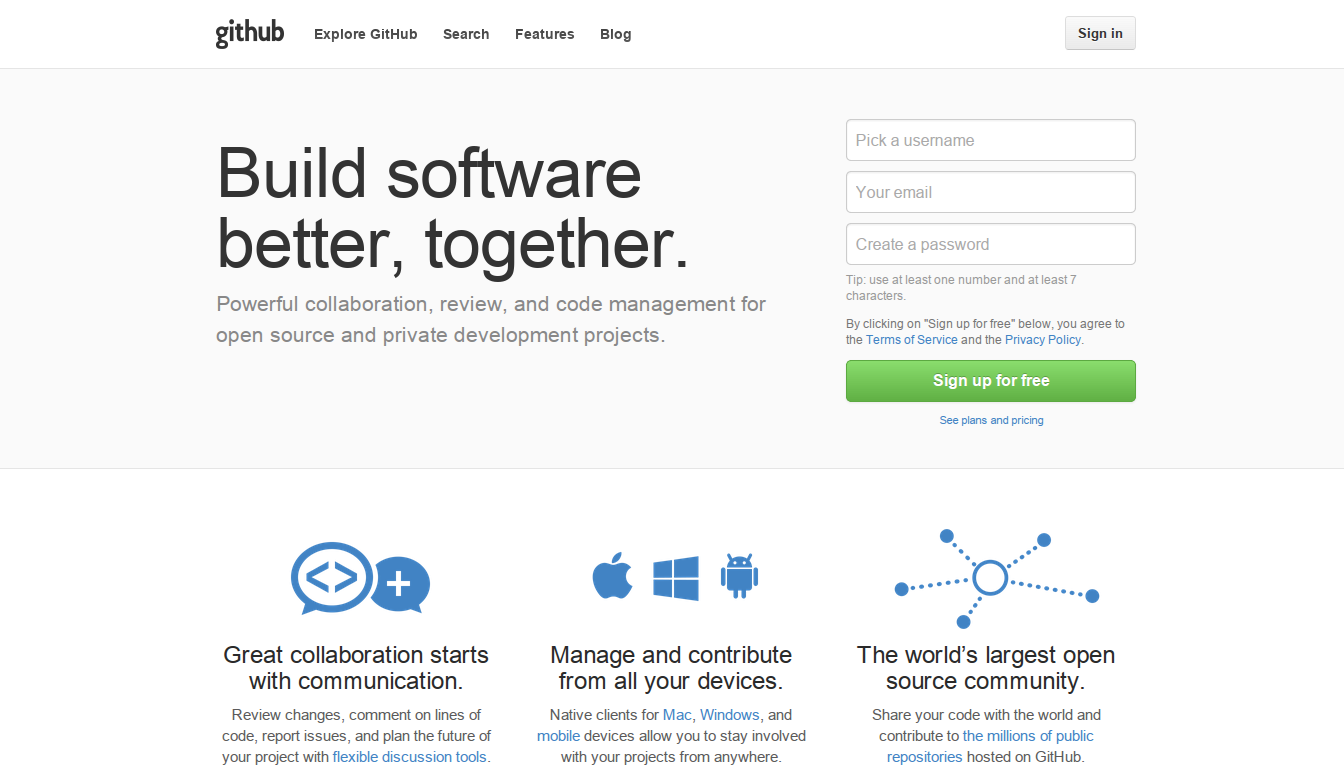
\includegraphics[width=11cm]{images/wui-example.png}
    \caption{Příklad webového uživatelského rozhraní (TODO: zdroj -- github.com).}
\end{figure}

Mezi hlavní výhody webových aplikací patří relativně jednoduchá udržovatelnost a flexibilita. Tyto vlastnosti jsou dány povahou klient--server modelu. Jedná se o síťovou architekturu, která rozlišuje klienta (uživatele) a server (aplikaci). Klient--server model umožňuje vývojářům udržovat pouze jednu verzi aplikace, která je multiplatformní a často daleko bezpečnější a spolehlivější. Nevýhodou je nižší dostupnost a vyšší odezva, která je dána kvalitou síťového (Internetového) připojení.

\section{Proces tvorby uživatelského rozhraní}
\label{sec:process}

\begin{quote}
\uv{Proces tvorby uživatelského rozhraní je zdokumentovaný postup, který je nutné absolvovat pro dokončení typického uživatelského rozhraní.}
\end{quote}

\noindent
Vývoj každého systému prochází několika fázemi, které se většinou překrývají z důvodu spolupráce vývojářů, designérů a analytiků. Tyto fáze lze rozdělit na čtyři části.

\begin{enumerate}[leftmargin=1cm]
    \item \textbf{Plánování}\\
          Zahrnuje analýzu požadavků klienta a cílové skupiny uživatelů. Dále tato fáze zahrnuje výběr programovacího jazyka, knihoven a dalších nástrojů, které budou použity pro implementaci.

    \item \textbf{Design}\\
          Informace shromážděné z předchozího stádia jsou sepsány a analyzovány. Návrh zahrnuje vývoj struktury a vizuální podoby aplikace a je obvykle rozdělen do tří částí---vytvoření drátěného modelu (anglicky \textit{Wireframe}), grafického návrhu a kódování šablon. Tyto kroky mají za úkol podrobněji specifikovat požadavky klienta a odhalit nejasnosti v zadání. Návrh probíhá převážně paralelně s vývojem.

    \item \textbf{Vývoj}\\
          V této fázi jsou požadované funkce systému implementovány za použití ustanovených technologií a knihoven. Vývoj zahrnuje verifikaci požadavků, integraci grafických návrhů do systému a testování celého systému včetně použitelnosti.

    \item \textbf{Spuštění}\\
           Jedná se o poslední fázi, která prochází nejdelším cyklem. Aplikace je nasazena na produkci. Tento krok je důležitý jednak z důvodů nepředvídatelného chování aplikace na serveru, především však z důvodu hlubšího testování koncovými uživateli.

\end{enumerate}

Tvorba uživatelského rozhraní je provázána se všemi těmito fázemi a zahrnuje několik aktivit, které vyžadují práci s různými nástroji a technologiemi. Tyto aktivity vyžadují rozdílné znalosti a jsou často rozděleny mezi specificky zaměřené specialisty.

\subsection{Tvorba drátěného modelu}
\label{sec:wireframing}

Webový drátěný model (anglicky \textit{wireframe}) je zjednodušená kresba, která reprezentuje rozmístění prvků a komponent webové stránky; prezentuje strukturální úroveň. Tvorba drátěného modelu zaujímá místo již na začátku životního cyklu projektu a slouží pro zachycení základní struktury stránky. Úkol drátěného modelu je poskytnout vizuální porozumění stránky již na počátku tvorby uživatelského rozhraní.

\begin{figure}[htbp]
    \centering
    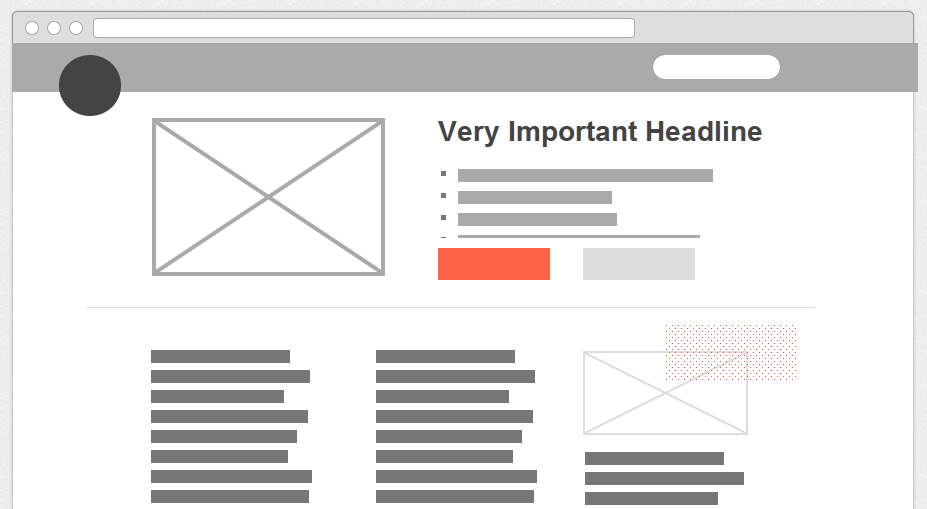
\includegraphics[width=11cm]{images/wireframe-example.png}
    \caption{Příklad drátěného modelu (TODO: zdroj -- wireframe.cc).}
\end{figure}

Výhodou drátěných modelů je jednoduchá přizpůsobitelnost potřebám klienta a jasně definovaná kostra, která zajišťuje sebedůvěru designera. V pozdějších fázích projektu by se neměl drátěný model nijak měnit a měl by odpovídat grafickému návrhu.

\subsection{Tvorba grafického návrhu}
\label{sec:designing}

Grafický návrh poskytuje vizuální podobu webové aplikace; reprezentuje aplikaci v podobě, ve které bude prezentována uživateli. Tato fáze zahrnuje výběr grafických a typografických prvků. Mezi grafické prvky obyčejně patří kombinace barev, obrázků, tvar tlačítek apod. Typografické prvky zahrnují především organizaci písma -- volbu řezů a rodin písma pro odlišení jednotlivých částí webové stránky. Dále zahrnují velikosti odstavců, odrážky, řádkování atd.

\subsection{Kódování}
\label{sec:coding}

V tomto stádiu přichází na řadu rozřezání a kódování grafického návrhu. Kódování probíhá v HTML (HyperText Markup Language) a CSS (Cascading Style Sheets). Kód by měl být psán s ohledem na W3C standard (World Wide Web Consortium) a měl by dodržovat osvědčené postupy pro zvýšení čitelnosti a podpory všech nejpoužívanějších prohlížečů.

